The official \EasyCrypt installation instructions are available on the \hyperref{https://github.com/EasyCrypt/easycrypt}{github}{ec}{EasyCrypt GitHub} repository. We provides a summary of these instructions, with a particular focus on their integration with the \hyperref{https://www.gnu.org/software/emacs/}{site}{emacs}{Emacs} text editor.\par
\EasyCrypt can operate in batch mode from the shell (command line) to check individual \texttt{.ec} files. However, interactive proof construction is conducted within \Emacs, utilizing the generic interface \ProofGeneral, which acts as a mediator between \Emacs and \EasyCrypt, the latter running as a sub-process of Emacs.

These instructions are aligned with the following software versions:
\begin{itemize}
	\item \OCaml compiler version 5.1.1
	\item \WhyThree version 1.7.2
	\item \AltErgo version 2.5.2
\end{itemize}
\EasyCrypt is implemented in \OCaml. \WhyThree serves as the interface to \SMT solvers used by \EasyCrypt, and \AltErgo is one of the \SMT solvers required for its operation.

\subsection*{Installing Emacs}
You'll first need to make sure autoconf is already installed on your system. Type which autoconf to find out.
\begin{lstlisting}[style=normal]
@:~$ sudo apt-get install autoconf
\end{lstlisting}
\begin{lstlisting}[style=normal]
@:~$ sudo apt-get install autoconf
\end{lstlisting}

\subsection*{Installing EasyCrypt}
\begin{itemize}
	\item \texttt{opam init} : creates .opam sub-directory of your home directory
	\item \texttt{eval \$(opam env)} : updates environment variables in current shell
\end{itemize}
\begin{lstlisting}[style=normal]
@:~$ sudo apt-get install opam
@:~$ opam init
@:~$ eval $(opam env)
\end{lstlisting}
\begin{itemize}
\item \texttt{opam switch create 5.1.1} : say which version of OCaml compiler to build
\end{itemize}
\begin{lstlisting}[style=normal]
@:~$ opam switch create 5.1.1
<><> Processing actions <><><><><><><><><><><><><><><><><><><><><><><><><><><>
* installed base-bigarray.base
...
Done.
@:~$ eval $(opam env)
\end{lstlisting}


\begin{lstlisting}[style=normal]
@:~$ opam pin -yn add easycrypt https://github.com/EasyCrypt/easycrypt.git
Package easycrypt does not exist, create as a NEW package? [Y/n] y
[easycrypt.~dev] synchronised (git+https://github.com/EasyCrypt/easycrypt.git)
easycrypt is now pinned to git+https://github.com/EasyCrypt/easycrypt.git (version ~dev)
@:~$ opam install --deps-only easycrypt
<><> Processing actions <><><><><><><><><><><><><><><><><><><><><><><><><><><>
[easycrypt.~dev] synchronised (no changes)

The following actions will be performed:
* install conf-gmp          4
...
* installed why3.1.7.1
Done.
@:~$ eval $(opam env)
\end{lstlisting}

\begin{lstlisting}[style=normal]
@:~$ CHECK_IF_PREINSTALLED=false opam install --deps-only easycrypt
[NOTE] It seems you have not updated your repositories for a while. Consider
updating them with:
opam update

<><> Synchronising pinned packages ><><><><><><><><><><><><><><><><><><><><><>
[easycrypt.~dev] synchronised (no changes)

Nothing to do.
\end{lstlisting}

\newpage
\begin{lstlisting}[style=normal]
@:~$ opam pin why3 1.7.1
@:~$ why3 --version
Why3 platform, version 1.7.1
@:~$ alt-ergo --version
v2.5.2
\end{lstlisting}

\begin{lstlisting}[style=normal]
@:~$ opam install easycrypt
@:~$ eval $(opam env)
\end{lstlisting}

There are binaries at this URL \url{https://github.com/Z3Prover/z3/releases/tag/z3-4.12.4}. If you need to build it from source, there are source archives available, too. Assuming you have the binary distribution, put the whole directory somewhere, and update your shell's startup script to add its bin directory to the PATH environment variable. Run which z3 while not in the Z3 bin directory to verify that you have set up PATH correctly.
\[
\texttt{export PATH="/home/username/z3-4.12.4-x64-glibc-2.35/bin:\$PATH"}
\]
\begin{lstlisting}[style=normal]
@:~$ which z3
/home/username/z3-4.12.4-x64-glibc-2.35/bin/z3
\end{lstlisting}


\begin{lstlisting}[style=normal]
@:~$ opam install easycrypt
@:~$ eval $(opam env)
@:~$ which easycrypt
/home/username/.opam/5.1.1/bin/easycrypt
@:~$ easycrypt why3config
Executing: why3 config detect -C /home/username/.config/easycrypt/why3.conf
Found prover Alt-Ergo version 2.5.2, OK.
Found prover Alt-Ergo version 2.5.2 (alternative: BV)
Found prover Alt-Ergo version 2.5.2 (alternative: counterexamples)
Found prover CVC4 version 1.8 (alternative: strings+counterexamples)
Found prover CVC4 version 1.8 (alternative: strings)
Found prover CVC4 version 1.8 (alternative: counterexamples)
Found prover CVC4 version 1.8, OK.
Found prover Z3 version 4.12.4 (alternative: counterexamples)
Found prover Z3 version 4.12.4, OK.
Found prover Z3 version 4.12.4 (alternative: noBV)
Found prover Coq version 8.15.0, but no Why3 libraries were compiled for it
10 prover(s) added
Save config to /home/username/.config/easycrypt/why3.conf
\end{lstlisting}


\begin{lstlisting}[style=normal]
@:~$ touch .emacs
@:~$ emadcs .emacs
\end{lstlisting}
\begin{lstlisting}[style=normal]
(require 'package)
(add-to-list 'package-archives '("melpa" . "https://melpa.org/packages/") t)
(package-initialize)
\end{lstlisting}
\begin{figure}[h!]\centering
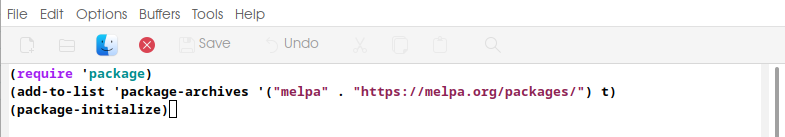
\includegraphics[width=\textwidth]{images/emacs/emacs1}
\end{figure}

%\subsection*{GNU Emacs}
%\addcontentsline{toc}{subsection}{GNU Emacs}
%\begin{center}
%	\begin{tikzpicture}[
%		timeline/.style={draw, thick, -{Latex[length=3mm]}},
%		event/.style={font=\footnotesize, anchor=west},
%		year/.style={anchor=east, font=\small\bfseries}
%		]
%		
%		% Timeline
%		\draw[timeline] (0, 0) -- (0, -7);
%		
%		% Events
%		\foreach \y/\version/\date in {
%			0.0/Emacs 29.4/Jun 22, 2024,
%			-1.0/Emacs 29.3/Mar 24, 2024,
%			-2.0/Emacs 29.2/Jan 18, 2024,
%			-3.0/Emacs 29.1/Jul 30, 2023,
%			-4.5/Emacs 28.2/Sep 12, 2022,
%			-5.5/Emacs 28.1/Apr 4, 2022
%		} {
%			\node[year\texttt{}] at (-0.5, \y) {\date};
%			\node[event] at (0.5, \y) {\version};
%		}
%		
%	\end{tikzpicture}
%\end{center}